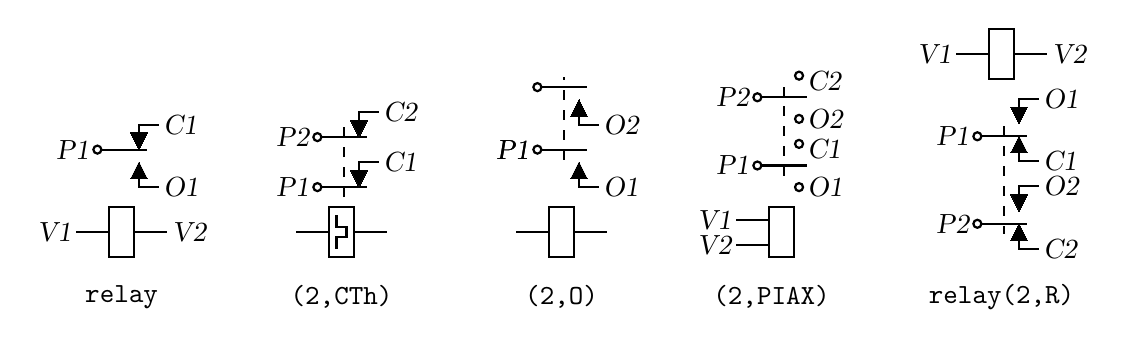
\begin{tikzpicture}[scale=2.54]
% dpic version 2020.03.01 option -g for TikZ and PGF 1.01
\ifx\dpiclw\undefined\newdimen\dpiclw\fi
\global\def\dpicdraw{\draw[line width=\dpiclw]}
\global\def\dpicstop{;}
\dpiclw=0.8bp
\dpiclw=0.8bp
\dpicdraw (0.291667,-0.227083)
 --(0.291667,-0.102083)
 --(0.166667,-0.102083)
 --(0.166667,-0.352083)
 --(0.291667,-0.352083)
 --(0.291667,-0.227083)\dpicstop
\dpicdraw (0.166667,-0.227083)
 --(0,-0.227083)\dpicstop
\dpicdraw (0.291667,-0.227083)
 --(0.458333,-0.227083)\dpicstop
\dpicdraw[fill=white](0.108333,0.185417) circle (0.007874in)\dpicstop
\dpicdraw (0.128333,0.185417)
 --(0.358333,0.185417)\dpicstop
\filldraw[line width=0bp](0.275,0.26875)
 --(0.316667,0.185417)
 --(0.358333,0.26875) --cycle\dpicstop
\dpicdraw (0.316667,0.197839)
 --(0.316667,0.310417)
 --(0.416667,0.310417)\dpicstop
\filldraw[line width=0bp](0.358333,0.039583)
 --(0.316667,0.122917)
 --(0.275,0.039583) --cycle\dpicstop
\dpicdraw (0.316667,0.110494)
 --(0.316667,-0.002083)
 --(0.416667,-0.002083)\dpicstop
\draw (0,-0.227083) node[left=-2bp]{\sl V1};
\draw (0.458333,-0.227083) node[right=-2bp]{\sl V2};
\draw (0.088333,0.185417) node[left=-2bp]{\sl P1};
\draw (0.416667,-0.002083) node[right=-2bp]{\sl O1};
\draw (0.416667,0.310417) node[right=-2bp]{\sl C1};
\draw (0.229167,-0.552083) node(S){\tt relay};
\dpicdraw (1.391667,-0.227083)
 --(1.391667,-0.102083)
 --(1.266667,-0.102083)
 --(1.266667,-0.352083)
 --(1.391667,-0.352083)
 --(1.391667,-0.227083)\dpicstop
\dpicdraw (1.266667,-0.227083)
 --(1.1,-0.227083)\dpicstop
\dpicdraw (1.391667,-0.227083)
 --(1.558333,-0.227083)\dpicstop
\dpicdraw (1.304167,-0.14375)
 --(1.304167,-0.202083)
 --(1.354167,-0.202083)
 --(1.354167,-0.252083)
 --(1.304167,-0.252083)
 --(1.304167,-0.310417)\dpicstop
\dpicdraw[fill=white](1.208333,-0.002083) circle (0.007874in)\dpicstop
\dpicdraw (1.228333,-0.002083)
 --(1.458333,-0.002083)\dpicstop
\filldraw[line width=0bp](1.375,0.08125)
 --(1.416667,-0.002083)
 --(1.458333,0.08125) --cycle\dpicstop
\dpicdraw (1.416667,0.010339)
 --(1.416667,0.122917)
 --(1.516667,0.122917)\dpicstop
\dpicdraw[fill=white](1.208333,0.247917) circle (0.007874in)\dpicstop
\dpicdraw (1.228333,0.247917)
 --(1.458333,0.247917)\dpicstop
\filldraw[line width=0bp](1.375,0.33125)
 --(1.416667,0.247917)
 --(1.458333,0.33125) --cycle\dpicstop
\dpicdraw (1.416667,0.260339)
 --(1.416667,0.372917)
 --(1.516667,0.372917)\dpicstop
\dpicdraw[dash pattern=on 0.05in off 0.05in](1.343333,-0.052083)
 --(1.343333,0.297917)\dpicstop
\draw (1.188333,-0.002083) node[left=-2bp]{\sl P1};
\draw (1.516667,0.122917) node[right=-2bp]{\sl C1};
\draw (1.188333,0.247917) node[left=-2bp]{\sl P2};
\draw (1.516667,0.372917) node[right=-2bp]{\sl C2};
\draw (1.329167,-0.552083) node{\tt (2,CTh)};
\dpicdraw (2.491667,-0.227083)
 --(2.491667,-0.102083)
 --(2.366667,-0.102083)
 --(2.366667,-0.352083)
 --(2.491667,-0.352083)
 --(2.491667,-0.227083)\dpicstop
\dpicdraw (2.366667,-0.227083)
 --(2.2,-0.227083)\dpicstop
\dpicdraw (2.491667,-0.227083)
 --(2.658333,-0.227083)\dpicstop
\dpicdraw[fill=white](2.308333,0.185417) circle (0.007874in)\dpicstop
\dpicdraw (2.328333,0.185417)
 --(2.558333,0.185417)\dpicstop
\filldraw[line width=0bp](2.558333,0.039583)
 --(2.516667,0.122917)
 --(2.475,0.039583) --cycle\dpicstop
\dpicdraw (2.516667,0.110494)
 --(2.516667,-0.002083)
 --(2.616667,-0.002083)\dpicstop
\dpicdraw[fill=white](2.308333,0.497917) circle (0.007874in)\dpicstop
\dpicdraw (2.328333,0.497917)
 --(2.558333,0.497917)\dpicstop
\filldraw[line width=0bp](2.558333,0.352083)
 --(2.516667,0.435417)
 --(2.475,0.352083) --cycle\dpicstop
\dpicdraw (2.516667,0.422994)
 --(2.516667,0.310417)
 --(2.616667,0.310417)\dpicstop
\dpicdraw[dash pattern=on 0.05in off 0.05in](2.443333,0.135417)
 --(2.443333,0.547917)\dpicstop
\draw (2.288333,0.185417) node[left=-2bp]{\sl P1};
\draw (2.616667,-0.002083) node[right=-2bp]{\sl O1};
\draw (2.288333,0.185417) node[left=-2bp]{\sl P1};
\draw (2.616667,0.310417) node[right=-2bp]{\sl O2};
\draw (2.429167,-0.552083) node{\tt (2,O)};
\dpicdraw (3.591667,-0.227083)
 --(3.591667,-0.102083)
 --(3.466667,-0.102083)
 --(3.466667,-0.352083)
 --(3.591667,-0.352083)
 --(3.591667,-0.227083)\dpicstop
\dpicdraw (3.466667,-0.164583)
 --(3.3,-0.164583)\dpicstop
\dpicdraw (3.466667,-0.289583)
 --(3.3,-0.289583)\dpicstop
\dpicdraw[fill=white](3.408333,0.105972) circle (0.007874in)\dpicstop
\dpicdraw[fill=white](3.616667,0.214028) circle (0.007874in)\dpicstop
\dpicdraw[fill=white](3.616667,-0.002083) circle (0.007874in)\dpicstop
\dpicdraw (3.428333,0.105972)
 --(3.658333,0.105972)\dpicstop
\dpicdraw[fill=white](3.408333,0.447083) circle (0.007874in)\dpicstop
\dpicdraw[fill=white](3.616667,0.555139) circle (0.007874in)\dpicstop
\dpicdraw[fill=white](3.616667,0.339028) circle (0.007874in)\dpicstop
\dpicdraw (3.428333,0.447083)
 --(3.658333,0.447083)\dpicstop
\dpicdraw[dash pattern=on 0.05in off 0.05in](3.543333,0.055972)
 --(3.543333,0.497083)\dpicstop
\draw (3.3,-0.164583) node[left=-2bp]{\sl V1};
\draw (3.3,-0.289583) node[left=-2bp]{\sl V2};
\draw (3.388333,0.105972) node[left=-2bp]{\sl P1};
\draw (3.636667,-0.002083) node[right=-2bp]{\sl O1};
\draw (3.636667,0.186354) node[right=-2bp]{\sl C1};
\draw (3.388333,0.447083) node[left=-2bp]{\sl P2};
\draw (3.636667,0.339028) node[right=-2bp]{\sl O2};
\draw (3.636667,0.527465) node[right=-2bp]{\sl C2};
\draw (3.479167,-0.552083) node{\tt (2,PIAX)};
\dpicdraw (4.691667,0.664583)
 --(4.691667,0.789583)
 --(4.566667,0.789583)
 --(4.566667,0.539583)
 --(4.691667,0.539583)
 --(4.691667,0.664583)\dpicstop
\dpicdraw (4.566667,0.664583)
 --(4.4,0.664583)\dpicstop
\dpicdraw (4.691667,0.664583)
 --(4.858333,0.664583)\dpicstop
\dpicdraw[fill=white](4.508333,0.252083) circle (0.007874in)\dpicstop
\dpicdraw (4.528333,0.252083)
 --(4.758333,0.252083)\dpicstop
\filldraw[line width=0bp](4.758333,0.16875)
 --(4.716667,0.252083)
 --(4.675,0.16875) --cycle\dpicstop
\dpicdraw (4.716667,0.239661)
 --(4.716667,0.127083)
 --(4.816667,0.127083)\dpicstop
\filldraw[line width=0bp](4.675,0.397917)
 --(4.716667,0.314583)
 --(4.758333,0.397917) --cycle\dpicstop
\dpicdraw (4.716667,0.327006)
 --(4.716667,0.439583)
 --(4.816667,0.439583)\dpicstop
\dpicdraw[fill=white](4.508333,-0.185417) circle (0.007874in)\dpicstop
\dpicdraw (4.528333,-0.185417)
 --(4.758333,-0.185417)\dpicstop
\filldraw[line width=0bp](4.758333,-0.26875)
 --(4.716667,-0.185417)
 --(4.675,-0.26875) --cycle\dpicstop
\dpicdraw (4.716667,-0.197839)
 --(4.716667,-0.310417)
 --(4.816667,-0.310417)\dpicstop
\filldraw[line width=0bp](4.675,-0.039583)
 --(4.716667,-0.122917)
 --(4.758333,-0.039583) --cycle\dpicstop
\dpicdraw (4.716667,-0.110494)
 --(4.716667,0.002083)
 --(4.816667,0.002083)\dpicstop
\dpicdraw[dash pattern=on 0.05in off 0.05in](4.643333,0.302083)
 --(4.643333,-0.235417)\dpicstop
\draw (4.4,0.664583) node[left=-2bp]{\sl V1};
\draw (4.858333,0.664583) node[right=-2bp]{\sl V2};
\draw (4.488333,0.252083) node[left=-2bp]{\sl P1};
\draw (4.816667,0.439583) node[right=-2bp]{\sl O1};
\draw (4.816667,0.127083) node[right=-2bp]{\sl C1};
\draw (4.488333,-0.185417) node[left=-2bp]{\sl P2};
\draw (4.816667,0.002083) node[right=-2bp]{\sl O2};
\draw (4.816667,-0.310417) node[right=-2bp]{\sl C2};
\draw (4.629167,-0.552083) node{\tt relay(2,R)};
\end{tikzpicture}
\vspace*{-0.5\baselineskip}
